% Modified based on Xiaoming Sun's template
\documentclass{article}
\usepackage{amsmath,amsfonts,amsthm,amssymb}
\usepackage{setspace}
\usepackage{fancyhdr}
\usepackage{lastpage}
\usepackage{extramarks}
\usepackage{chngpage}
\usepackage{soul,color}
\usepackage{graphicx,float,wrapfig}

\usepackage{hyperref}
\hypersetup{
    colorlinks=true,
    linkcolor=blue,
    filecolor=magenta,      
    urlcolor=cyan,
}

\newcommand{\Class}{Mathematics for Computer Science}

% Homework Specific Information. Change it to your own
\newcommand{\Title}{Homework 2}

% In case you need to adjust margins:
\topmargin=-0.45in      %
\evensidemargin=0in     %
\oddsidemargin=0in      %
\textwidth=6.5in        %
\textheight=9.0in       %
\headsep=0.25in         %

% Setup the header and footer
\pagestyle{fancy}                                                       %
\chead{\Title}  %
\rhead{\firstxmark}                                                     %
\lfoot{\lastxmark}                                                      %
\cfoot{}                                                                %
\rfoot{Page\ \thepage\ of\ \protect\pageref{LastPage}}                          %
\renewcommand\headrulewidth{0.4pt}                                      %
\renewcommand\footrulewidth{0.4pt}                                      %

%%%%%%%%%%%%%%%%%%%%%%%%%%%%%%%%%%%%%%%%%%%%%%%%%%%%%%%%%%%%%
% Some tools
\newcommand{\enterProblemHeader}[1]{\nobreak\extramarks{#1}{#1 continued on next page\ldots}\nobreak%
                                    \nobreak\extramarks{#1 (continued)}{#1 continued on next page\ldots}\nobreak}%
\newcommand{\exitProblemHeader}[1]{\nobreak\extramarks{#1 (continued)}{#1 continued on next page\ldots}\nobreak%
                                   \nobreak\extramarks{#1}{}\nobreak}%

\newcommand{\homeworkProblemName}{}%
\newcounter{homeworkProblemCounter}%
\newenvironment{homeworkProblem}[1][Problem \arabic{homeworkProblemCounter}]%
  {\stepcounter{homeworkProblemCounter}%
   \renewcommand{\homeworkProblemName}{#1}%
   \section*{\homeworkProblemName}%
   \enterProblemHeader{\homeworkProblemName}}%
  {\exitProblemHeader{\homeworkProblemName}}%

\newcommand{\homeworkSectionName}{}%
\newlength{\homeworkSectionLabelLength}{}%
\newenvironment{homeworkSection}[1]%
  {% We put this space here to make sure we're not connected to the above.

   \renewcommand{\homeworkSectionName}{#1}%
   \settowidth{\homeworkSectionLabelLength}{\homeworkSectionName}%
   \addtolength{\homeworkSectionLabelLength}{0.25in}%
   \changetext{}{-\homeworkSectionLabelLength}{}{}{}%
   \subsection*{\homeworkSectionName}%
   \enterProblemHeader{\homeworkProblemName\ [\homeworkSectionName]}}%
  {\enterProblemHeader{\homeworkProblemName}%

   % We put the blank space above in order to make sure this margin
   % change doesn't happen too soon.
   \changetext{}{+\homeworkSectionLabelLength}{}{}{}}%

\newcommand{\Answer}{\ \\\textbf{Answer:} }
\newcommand{\Acknowledgement}[1]{\ \\{\bf Acknowledgement:} #1}

%%%%%%%%%%%%%%%%%%%%%%%%%%%%%%%%%%%%%%%%%%%%%%%%%%%%%%%%%%%%%


%%%%%%%%%%%%%%%%%%%%%%%%%%%%%%%%%%%%%%%%%%%%%%%%%%%%%%%%%%%%%
% Make title
\title{\textmd{\bf \Class: \Title}}
\date{March 8, 2019}
\author{Xingyu Su 2015010697}
%%%%%%%%%%%%%%%%%%%%%%%%%%%%%%%%%%%%%%%%%%%%%%%%%%%%%%%%%%%%%

\begin{document}
\begin{spacing}{1.1}
\maketitle \thispagestyle{empty}

%%%%%%%%%%%%%%%%%%%%%%%%%%%%%%%%%%%%%%%%%%%%%%%%%%%%%%%%%%%%%
% Begin edit from here

%%%%%%%%%%%%%%%%%%%%%%%%%%%%%%%%%%%%%%%%%%%%%%%%%%%%%%%%%%%%%
% HOMEWORK-2-LPV 3.8.8
\begin{homeworkProblem}[LPV 3.8.8]
Prove the following identities:
\begin{align*}
  \sum_{k=0}^{m}{(-1)^k\binom{n}{k}} = (-1)^m\binom{n-1}{m};\\
  \sum_{k=0}^n\binom{n}{k}\binom{k}{m}=\binom{n}{m}2^{n-m}.
\end{align*}

\Answer 

From Pascal Triangle, we have
\begin{equation*}
  \binom{n}{k}=\binom{n-1}{k-1}+\binom{n-1}{k}
\end{equation*}
\hspace{1em}
So we have:
\begin{align*}
  \sum_{k=0}^{m}{(-1)^k\binom{n}{k}}
    &=\binom{n}{0}-\binom{n}{1}+\binom{n}{2}-\binom{n}{3}+\cdots+(-1)^k\binom{n}{k} \\
    &=\binom{n-1}{0}-\left[\binom{n-1}{0}+\binom{n-1}{1}\right]+\left[\binom{n-1}{1}+\binom{n-1}{2}\right]-\cdots+(-1)^m\left[\binom{n-1}{m-1}+\binom{n-1}{m}\right] \\
    &=(-1)^m\binom{n-1}{m}
\end{align*}
\hspace{1em}
For the second identity, consider m is a non-negetive number. So when $k<m$, $\binom{k}{m}=0$, then:
\begin{equation*}
  \sum_{k=0}^n\binom{n}{k}\binom{k}{m} = \sum_{k=m}^n\binom{n}{k}\binom{k}{m}
\end{equation*}
\hspace{1em}
Easy to find:
\begin{align*}
  \binom{n}{k}\binom{k}{m} 
    &= \frac{n!}{k!(n-k)!}\frac{k!}{m!(k-m)!} \\
    &= \frac{n!}{(n-k)!(k-m)!m!} \\
    &= \frac{n!}{(n-m)!m!}\frac{(n-m)!}{(n-k)!(k-m)!} \\
    &= \binom{n-m}{k-m}\binom{n}{m}
\end{align*}
\hspace{1em}
So:
\begin{equation*}
\sum_{k=0}^n\binom{n}{k}\binom{k}{m}=\binom{n}{m}\sum_{k=m}^n\binom{n-m}{k-m} = \binom{n}{m}\sum_{i=0}^{n-m}\binom{n-m}{i}=\binom{n}{m}2^{n-m}
\end{equation*}
\end{homeworkProblem}
%%%%%%%%%%%%%%%%%%%%%%%%%%%%%%%%%%%%%%%%%%%%%%%%%%%%%%%%%%%%%


%%%%%%%%%%%%%%%%%%%%%%%%%%%%%%%%%%%%%%%%%%%%%%%%%%%%%%%%%%%%%
% HOMEWORK-2-LPV 3.8.12
\begin{homeworkProblem}[LPV 3.8.12]
Prove that
\begin{equation*}
  1+\binom{n}{1}2+\binom{n}{2}4+\cdots+\binom{n}{n-1}2^{n-1}+\binom{n}{n}2^n=3^n.
\end{equation*}
Try to find a combinatorial proof.

\Answer 

Consider $n=1$, obviously we have $1+\binom{1}{1}2=3=3^1$, equation is true. If the equation is true when $n=k-1$:
\begin{equation*}
  1+\binom{k-1}{1}2+\binom{k-1}{2}4+\cdots+\binom{k-1}{k-1}2^{k-1} = 3^{k-1}
\end{equation*}
\hspace{1em}
Then for $n=k$, we have:
\begin{align*}
  & 1+\binom{k}{1}2+\binom{k}{2}4+\cdots+\binom{k-1}{k-1}2^{k-1}+\binom{k}{k}2^{k} \\
    & = 1 + \left[\binom{k-1}{0}+\binom{k-1}{1}\right]2+\left[\binom{k-1}{1}+\binom{k-1}{2}\right]4+\cdots+\left[\binom{k-1}{k-1}+\binom{k-1}{k}\right]2^k \\
    & = 1+\binom{k-1}{1}2+\binom{k-1}{2}4+\cdots+\binom{k-1}{k-1}2^{k-1} + 2 +\binom{k-1}{1}4+\cdots+\binom{k-1}{k-1}2^{k} \\
    & = 3^{k-1}+2\times 3^{k-1} \\
    & = 3^k
\end{align*}
\hspace{1em}
So the equation is true for all $n=1,2,3,...$

\end{homeworkProblem}
%%%%%%%%%%%%%%%%%%%%%%%%%%%%%%%%%%%%%%%%%%%%%%%%%%%%%%%%%%%%%

%%%%%%%%%%%%%%%%%%%%%%%%%%%%%%%%%%%%%%%%%%%%%%%%%%%%%%%%%%%%%
% HOMEWORK-2-LPV 3.8.14
\begin{homeworkProblem}[LPV 3.8.14]
Let $n$ be a positive integer divisible by 3. Use Stirling’s formula to find the approximate value of $\binom{n}{n/3}$.

\Answer 

We know that:
\begin{equation*}
\binom{n}{n/3}=\frac{n!}{(n/3)!(2n/3)!}
\end{equation*}
\hspace{1em}
By the Stirling's formula, we have:
\begin{equation*}
n!\ \sim \sqrt{2\pi n}\left(\frac{n}{e}\right)^n, (n/3)!\ \sim \sqrt{2\pi n/3}\left(\frac{n/3}{e}\right)^{n/3}, (2n/3)!\ \sim \sqrt{4\pi n/3}\left(\frac{2n/3}{e}\right)^{2n/3},
\end{equation*}
\hspace{1em}
And so:
\begin{equation*}
  \binom{n}{n/3}
    =\frac{\sqrt{2\pi n}\left(\frac{n}{e}\right)^n}{\sqrt{2\pi n/3}\left(\frac{n/3}{e}\right)^{n/3} \sqrt{4\pi n/3}\left(\frac{2n/3}{e}\right)^{2n/3}} 
    =\frac{1}{2/3\sqrt{\pi n}\left(\frac{1}{3}\right)^n 2^{2n/3}} 
    =\frac{3}{2}\sqrt{\frac{1}{\pi n}} 3^n 2^{-\frac{2}{3}n}
\end{equation*}
\hspace{1em}
The comparison between the real value and its approxmation is shown in Figure 1.
\begin{figure}[ht]
  \centering
  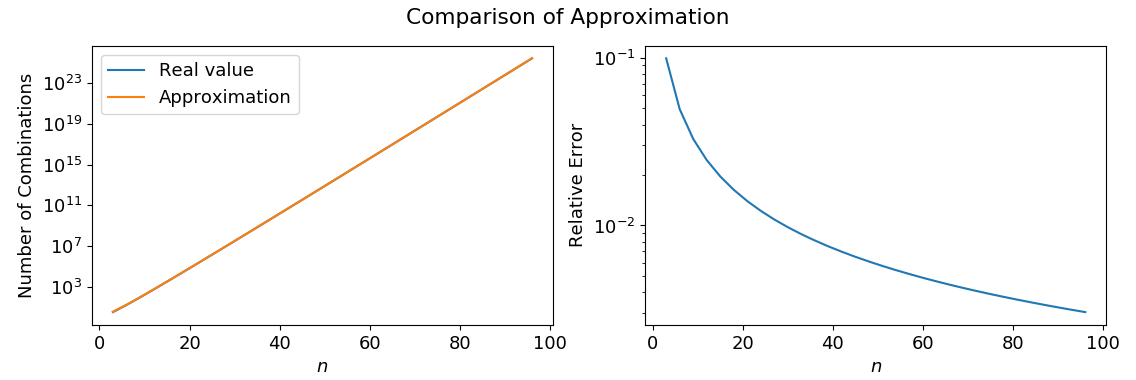
\includegraphics[width=1.0\linewidth]{figures/compare}
  \caption{Comparison of between approximation and real value with total number varies from 3 to 99.}
  \label{fig:compare}
\end{figure}

\end{homeworkProblem}
%%%%%%%%%%%%%%%%%%%%%%%%%%%%%%%%%%%%%%%%%%%%%%%%%%%%%%%%%%%%%


%%%%%%%%%%%%%%%%%%%%%%%%%%%%%%%%%%%%%%%%%%%%%%%%%%%%%%%%%%%%%
% HOMEWORK-2-LPV 4.3.7
\begin{homeworkProblem}[LPV 4.3.7]
How many subsets does the set $\{1, 2, \cdots , n\}$ have that contain no three consecutive integers? Find a recurrence.

\Answer 

Denote the sequence of integers as $A_n$. It's easy to find that $A_1 = 1$, $A_2 = 3$, $A_3 = 6$, $A_4=12$. And as shown in Figure 2, when $A_1, A_2, \cdots,A_n$ are known, we can get $A_{n+1}$ from previous values. (1) Consider the part of subsets without element $n+1$, this part counts to be $A_n$ obviously; and the part contains element $n+1$ can be divide into 2 parts: (2a) $A_n$ with $n+1$ which contains (2b) $A_{n-3}$ exception violating rules. So the recurrence can be written as:
\begin{equation*}
  A_{n+1} = 2A_n-A_{n-3}
\end{equation*}
\hspace{1em}
With this formula, we can get $A_5= 2A_4-A_1=23$, which is proved to be true after counting by hands.
\begin{figure}[ht]
  \centering
  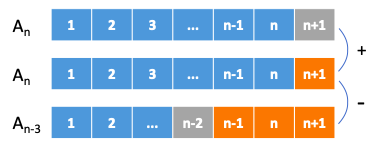
\includegraphics[width=0.5\linewidth]{figures/recurr}
  \caption{Demonstration of the recurrence of $A_n$.}
  \label{fig:recurr}
\end{figure}

\end{homeworkProblem}
%%%%%%%%%%%%%%%%%%%%%%%%%%%%%%%%%%%%%%%%%%%%%%%%%%%%%%%%%%%%%


%%%%%%%%%%%%%%%%%%%%%%%%%%%%%%%%%%%%%%%%%%%%%%%%%%%%%%%%%%%%%
% HOMEWORK-2-LPV 4.3.12
\begin{homeworkProblem}[LPV 4.3.12]
Recalling the Lucas numbers $L_n$ introduced in Exercise 4.3.2, prove the following identities:

(a) $ F_{2n}=F_nL_n;$

(b) $ 2F_{k+n}=F_kL_n+F_nL_k;$

(c) $ 2L_{k+n}=5F_kF_n+L_kL_n;$

(d) $ L_{4k}=L_{2k}^2-2;$

(e) $ L_{4k+2}=L_{2k+1}^2+2.$
\Answer 

From Exercise 4.3.2 we can easily know that:
\begin{equation*}
L_{n} = F_n+2F_{n-1}
\end{equation*}
\hspace{1em}
(a)
\begin{align*}
F_n L_n
  &=F_n(F_n+2F_{n-1}) \\
  &=F_n^2+2F_nF_{n-1}+F^2_{n-1}-F^2_{n-1} \\
  &=(F_n+F_{n-1})^2-F_{n-1}^2 \\
  &=F_{n+1}^2+F_{n}^2-F_n^2-F_{n-1}^2 \\
  &=F_{2n+1}-F_{2n-1} \\
  &=F_{2n}
\end{align*}
\hspace{2em}
(b) From identity (4.5) $F_{a+b+1}=F_{a+1}F_{b+1}+F_a F_b$, we can get:
\begin{align*}
  F_k L_n + F_n L_k 
    &=F_k(F_n+2F_{n-1})+F_n(F_k+2F_{k-1}) \\
    &=2F_k F_n+2F_{n-1}F_k+2F_{k-1}F_n +2F_{k-1}F_{n-1}-2F_{k-1}F_{n-1} \\
    &=2(F_k+F_{k+1})(F_n+F_{n-1})-2F_{k-1}F_{n-1} \\
    &=2(F_{k+1} F_{n+1}+F_k F_n-F_k F_n-F_{k-1}F_{n-1}) \\
    &=2(F_{k+n+1}-F_{k+n-1}) \\
    &=2F_{k+n}
\end{align*}
\hspace{2em}
(c)
\begin{align*}
  5F_k F_n +L_k L_n 
    &= 5F_k F_n + (F_k+2F_{k-1})(F_n+2F_{n-1}) \\
    &= 2(F_k F_n +F_{k-1}F_n+2F_{n-1}F_k)+4(F_k F_n+F_{k-1}F_{n-1}) \\
    &= 2F_{k+n}+4F_{k+n-1} \\
    &= 2L_{k+n}
\end{align*}
\hspace{2em}
(d) From (a) and identity (4.5), it's easy to get:
\begin{align*}
  L_{4k} 
    &= F_{4k}+2F_{4k-1} \\
    &= F_{2k}L_{2k}+2(F_{2k}F_{2k}+F_{2k-1}F_{2k-1}) \\
    &= L_{2k}^2-L_{2k}(F_{2k}+2F_{2k-1})+F_{2k}L_{2k}+2(F_{2k}F_{2k}+F_{2k-1}F_{2k-1})\\
    &= L_{2k}^2-2F_{2k}F_{2k-1}+2F_{2k}^2-2F_{2k-1}^2 \\
    &= L_{2k}^2+2F_{2k}^2-2F_{2k-1}F_{2k+1}
\end{align*}

\hspace{2em}
Denote $A_n = F_{n}^2-F_{n-1}F_{n+1}$, so:
\begin{align*}
  A_n 
    &= F_{n}^2-F_{n-1}F_{n+1} \\
    &= F_n^2-F_{n-1}(F_n+F_{n-1}) \\
    &= (F_n-F_{n-1})F_n-F_{n-1}^2 \\
    &= -(F_{n-1}^2 - F_{n-2}F_n) \\
    &=-A_{n-1} \\
    &= (-1)^{n-1} A_1
\end{align*}

\hspace{2em}
And $A_1 = F_1^2-F_0 F_2=1$, so:
\begin{equation*}
  L_{4k} = L_{2k}^2+2A_{2k}=L_{2k}^2+2(-1)^{2k-1}=L_{2k}^2-2
\end{equation*}

\hspace{2em}
(e) Similar to (d), we have:
\begin{equation*}
  L_{4k+2} = L_{2k+1}^2+2A_{2k+1}=L_{2k+1}^2+2(-1)^{2k}=L_{2k+1}^2+2
\end{equation*}
\end{homeworkProblem}
%%%%%%%%%%%%%%%%%%%%%%%%%%%%%%%%%%%%%%%%%%%%%%%%%%%%%%%%%%%%%


%%%%%%%%%%%%%%%%%%%%%%%%%%%%%%%%%%%%%%%%%%%%%%%%%%%%%%%%%%%%%
% HOMEWORK-2-LPV 4.3.14
\begin{homeworkProblem}[LPV 4.3.14]
\hspace{1.2em}
(a) Prove that every positive integer can be written as the sum of different Fibonacci numbers.

(b) Prove even more: every positive integer can be written as the sum of different Fibonacci numbers, so that no two consecutive Fibonacci numbers are used.

(c) Show by an example that the representation in (a) is not unique, but also prove that the more restrictive representation in (b) is.

\Answer 

(a) Consider positive integer $N$, when $N$ is equal to a Fibonacci number, the identity is obviously true. If for any $0<N<F_n$, the identity is true, and 
\begin{equation*}
  N=\sum_{i=1}^{n-1}a_i F_i, a_i \in \{0,1\}
\end{equation*}
So for bigger integer $F_n<N<F_{n+1}$, we can get:
\begin{equation*}
  N=F_n+\sum_{i=1}^{n-1}b_i F_i, b_i \in \{0,1\}
\end{equation*}
which means if first few integers satisfy the identity, then the identity is true for all integers. Since we have known that for $N=1,2,3,5,8...$, the identity is true. Then we can say  every positive integer can be written as the sum of different Fibonacci numbers.

(b) Similar to (a), we only need to prove that $\sum F_n+F_{n-2}+\cdots \geq F_{n+1}-1$, then for every integers between $F_{n}$ and $F_{n+1}$, the identity are true. Here are inductions:
\begin{equation*}
  F_1+F_3 = F_4,\ \text{then}\ F_1+F_3+F_5=F_4+F_5=F_6
\end{equation*}
\begin{equation*}
  \text{Known} \sum_{i=1}^{k}F_{2k-1}=F_{2k}, \text{then} \sum_{i=1}^{k+1}F_{2k-1}=F_{2k}+F_{2k+1} =F_{2k+1}
\end{equation*}
\begin{equation*}
  F_2+F_4 = F_5-1,\ \text{then}\ F_2+F_4+F_6=F_5-1+F_6=F_7-1
\end{equation*}
\begin{equation*}
  \text{Known} \sum_{i=1}^{k}F_{2k}=F_{2k+1}-1, \text{then} \sum_{i=1}^{k+1}F_{2k}=F_{2k+1}-1+F_{2k+2} =F_{2k+3}-1
\end{equation*}

So $\sum F_n+F_{n-2}+\cdots \geq F_{n+1}-1$ is true for all positive even numbers and odd numbers. Which in result proves the identity.

(c) An example: when $N=32$, there can be 2 ways to represent (a) as below
\begin{equation*}
  32 = 21 + 8 + 3 = 13 + 8 + 5 + 3 + 2 + 1
\end{equation*}
\hspace{1em}
But for representation in (b), there is only one exception that
\begin{equation*}
  F_{2k} = \sum_{i=1}^k F_{2k-1}
\end{equation*}
\hspace{1em}
And all integers left have only one way to get the identity true shown in (b).
\end{homeworkProblem}
%%%%%%%%%%%%%%%%%%%%%%%%%%%%%%%%%%%%%%%%%%%%%%%%%%%%%%%%%%%%%


%%%%%%%%%%%%%%%%%%%%%%%%%%%%%%%%%%%%%%%%%%%%%%%%%%%%%%%%%%%%%
% HOMEWORK-2-Special Problem 1
\begin{homeworkProblem}[Special Problem 1]
In class we considered a 3-Person Hat Problem in which each person can see the bits posted on the other two people’s foreheads and tries to guess the bit on his/her own forehead, but each person is permitted to make no guess; the team wins if (1) no one makes an incorrect guess, and (2) at least one person makes a correct guess. We discussed a strategy for the team with a probability 3/4 to win.

\textit{Question:} Give a rigorous proof that this is the best strategy possible. That is, no strategy for the team can win with probability higher than 3/4. Your model should be general enough to include strategies with randomized moves. (Recall that in class, we mentioned a particular strategy in which one person always make a random guess (0 or 1) and the other two don’t speak.)

\textbf{Remarks} You should first define a mathematical model. Define a probability space, how any strategy is specified precisely, and how to define win as an event for the strategy. This allows you to define what the term best strategy means.

\Answer 

The state space should be:
\begin{align*}
  & \{0,0,0\}, \ \{0,0,1\}, \ \{0,1,0\}, \ \{0,1,1\},\\
  & \{1,0,0\}, \ \{1,0,1\}, \ \{1,1,0\}, \ \{1,1,1\}
\end{align*}

\hspace{1em}
And probability for each state is all ${1/8}$. The strategy to win ${3/4}$ conditions is:

\hspace{2em}
(1) If first person sees one type of bits, he guess the other type. The other two partners will know their bits.

\hspace{2em}
(2)If first person sees two type of bits, he makes no guess. Since the other two will know each others' bit, then they can guess for themselves.

\hspace{1em} 
Consider the infomation passed from the first person, we can know for sure that \textbf{he can not make sure what type of bit he has in every state}. And \textbf{if he always make no guess, he brings nothing to the other two}. Which means he can only \textbf{make no guess in at most half of states to pass infomation}, and \textbf{for the other half, he can only make a guess which can wins in at most half of states left}.

\hspace{1em}
The proof is not rigorous enough, but it explains well for me.

\end{homeworkProblem}
%%%%%%%%%%%%%%%%%%%%%%%%%%%%%%%%%%%%%%%%%%%%%%%%%%%%%%%%%%%%%


%%%%%%%%%%%%%%%%%%%%%%%%%%%%%%%%%%%%%%%%%%%%%%%%%%%%%%%%%%%%%
% HOMEWORK-2-Special Problem 2
\begin{homeworkProblem}[Special Problem 2]
We discussed in class a game of ”Finding your IDs” for n students, using a cycle-following strategy for all the students. Let $g(n)$ be the probability of winning in this game, i.e. all students succeed in finding their ID.

(a) Give an explicit mathematical formula for $g(n)$.

(b) Determine the value of $\lim_{n\to \infty}g(n)$.

(c) Let us consider a modified game, in which each student is only allowed to search through $n/3$ boxes (instead of $n/2$). Let $h(n)$ be the probability of winning. Determine the value of $\lim_{n\to\infty} h(n)$.

\Answer 

(a) Since each student have half probability to get his ID correct, then $g(n)=(\frac{1}{2})^n$

(b) $\lim_{n\to\infty}g(n)=\lim_{n\to\infty}(\frac{1}{2})^n=0$

(c) Similarly, $h(n)=(\frac{1}{3})^n$, $\lim_{n\to\infty}h(n)=\lim_{n\to\infty}(\frac{1}{3})^n=0$

\end{homeworkProblem}
%%%%%%%%%%%%%%%%%%%%%%%%%%%%%%%%%%%%%%%%%%%%%%%%%%%%%%%%%%%%%


%%%%%%%%%%%%%%%%%%%%%%%%%%%%%%%%%%%%%%%%%%%%%%%%%%%%%%%%%%%%%
% HOMEWORK-2-Special Problem 3
\begin{homeworkProblem}[Special Problem 3]
In a New Year’s party with $2n$ people, $k$ random names are picked to receive gifts. Assume that these $2n$ people are actually $n$ husband-wife couples. Let $r_{n,k}$ be the probability that at least for one couple, both husband and wife win gifts.

(a) Give a mathematical formula for $r_{n,k}$.

(b) Determine the value of $\lim_{n\to\infty}r_{n,\sqrt{n}}$ .

\Answer 

(a) The opposite condition is that all k persons belong to different couples. So:
\begin{align*}
  & if\ k\leq n, r_{n,k} = 1-\frac{C_{n}^{k} 2^k}{C_{2n}^{k}} \\
  & else, \ r_{n,k}=1
\end{align*}

\hspace{1em}
(b) For ${n,k}$
\begin{equation*}
1-\frac{C_{n}^{k} 2^k}{C_{2n}^{k}} = 1-\frac{n!2^k (2n-k)!}{(2n)!(n-k)!}
\end{equation*}

\hspace{1em}
And with $k=\sqrt{n}$, Stirling's formula $n!\sim \sqrt{2\pi n}(\frac{n}{e})^n$, we have:
\begin{align*}
  \lim_{n\to\infty}{r_{n,\sqrt{n}}} 
    &= 1-\lim_{n\to\infty}\frac{\sqrt{2\pi n}\left(\frac{n}{e}\right)^n\sqrt{2\pi (2n-\sqrt{n})}\left(\frac{2n-\sqrt{n}}{e}\right)^{2n-\sqrt{n}}}{\sqrt{2\pi 2n}\left(\frac{2n}{e}\right)^{2n}\sqrt{2\pi(n-\sqrt{n})}\left(\frac{n-\sqrt{n}}{e}\right)^{n-\sqrt{n}}} \\
    &= 1-\lim_{n\to\infty}\sqrt{\frac{2\sqrt{n}-1}{2\sqrt{n}-2}}\left(\frac{2\sqrt{n}-1}{2\sqrt{n}-2}\right)^{n-\sqrt{n}}\left(1-\frac{1}{2\sqrt{n}}\right)^{n}
\end{align*}

\hspace{1em}
Denote $\sqrt{n}$ as $x$, then
\begin{equation*}
  \lim_{n\to\infty}{r_{n,\sqrt{n}}} = 1-\lim_{x\to\infty}\left(\frac{2x-1}{2x-2}\right)^{x^2-x+\frac{1}{2}}\left(1-\frac{1}{2x}\right)^{x^2} \triangleq 1-A
\end{equation*}
\begin{align*}
  \ln{A} 
    &= \lim_{x\to\infty}\left(x^2-x+\frac{1}{2}\right)\ln{\left(1+\frac{1}{2x-2}\right)}+\lim_{x\to\infty}x^2\ln\left(1-\frac{1}{2x}\right) \\
    &= \lim_{x\to\infty}\left(-x+\frac{1}{2}\right)\ln{\left(1+\frac{1}{2x-2}\right)}+\lim_{x\to\infty}x^2\ln{\left(1+\frac{1}{2x-2}\right)\left(1-\frac{1}{2x}\right)}
\end{align*}
\hspace{1em}
First part:
\begin{align*}
  \lim_{x\to\infty}\left(-x+\frac{1}{2}\right)\ln{\left(1+\frac{1}{2x-2}\right)} 
    &= -\frac{1}{2}\lim_{c\to\infty}(c+1)\ln(1+1/c) \\
    &= -\frac{1}{2}\lim_{c\to\infty}\frac{\partial \ln(1+1/c)}{\partial c}/\frac{\partial \frac{1}{c+1}}{\partial c} \\
    &= -\frac{1}{2}\lim_{c\to\infty}\frac{c+1}{c}\\
    &= -\frac{1}{2}
\end{align*}

\hspace{1em}
Second part:
\begin{align*}
  \lim_{x\to\infty}x^2\ln{\left(1+\frac{1}{2x-2}\right)\left(1-\frac{1}{2x}\right)} 
    &= \lim_{x\to\infty}x^2\ln\left(1+\frac{1}{4x(x-1)}\right) \\
    &= \lim_{x\to\infty}\frac{\frac{\partial \ln(1+\frac{1}{4x(x-1)})}{\partial x}}{\frac{\partial \frac{1}{x^2}}{\partial x}} \\
    &= \lim_{x\to\infty}\frac{x^2}{2(x-1)(2x-1)} \\
    &= \frac{1}{4}
\end{align*}

\hspace{1em}
So:
\begin{equation*}
\lim_{n\to\infty}{r_{n,\sqrt{n}}}=1-e^{\ln A}=1-e^{-\frac{1}{2}+\frac{1}{4}}=1-e^{-\frac{1}{4}}
\end{equation*}

\hspace{1em}
And Figure 3 shows the convergence between of $r_{n,\sqrt{n}}$ and $1-e^{-\frac{1}{4}}$.
\begin{figure}[ht]
  \centering
  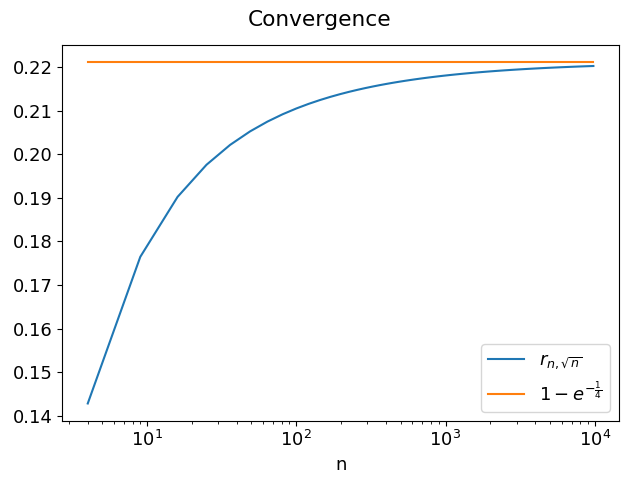
\includegraphics[width=0.5\linewidth]{figures/conver}
  \caption{Demonstration of the convergence between of $r_{n,\sqrt{n}}$ and $1-e^{-\frac{1}{4}}$.}
  \label{fig:conver}
\end{figure}

\end{homeworkProblem}
%%%%%%%%%%%%%%%%%%%%%%%%%%%%%%%%%%%%%%%%%%%%%%%%%%%%%%%%%%%%%

% ACKNOWLEGEMENT
\Acknowledgement

[1] Thanks to \href{https://github.com/jiweiqi}{Weiqi Ji} for discussing about SP3(b).


% End edit to here
%%%%%%%%%%%%%%%%%%%%%%%%%%%%%%%%%%%%%%%%%%%%%%%%%%%%%%%%%%%%%

\end{spacing}
\end{document}

%%%%%%%%%%%%%%%%%%%%%%%%%%%%%%%%%%%%%%%%%%%%%%%%%%%%%%%%%%%%%
